\documentclass[11pt,spanish]{article}


\usepackage[utf8]{inputenc}
\usepackage{subfiles}
\usepackage{biblatex}
\addbibresource{references.bib}
\usepackage{multicol}
\usepackage{amsfonts}
\usepackage{blindtext}
\usepackage{mathrsfs}
\usepackage{amsmath}
\usepackage{siunitx}
\usepackage{centernot}
\usepackage[shortlabels]{enumitem}
\usepackage{subfig}
\usepackage{datetime}
\usepackage{listingsutf8}
\usepackage[spanish]{babel}
\usepackage{tikz}
\usepackage{hyperref}
\usepackage[vlined,ruled,linesnumbered]{algorithm2e}
\usepackage{listings}
\usepackage{float}
\usepackage{url}
\usepackage{csquotes}
\usepackage{fourier} %font
\usepackage[top=2cm, bottom=2cm, left=2.5cm, right=2.5cm]{geometry}
\usepackage{pgfplots}
\usepackage{fancyhdr}
\usepackage{mdframed}
\usepackage{tikzducks}
\usepackage[nameinlink]{cleveref}
\usepackage{epigraph} 

\pgfplotsset{compat=1.18}

\usetikzlibrary{shapes.arrows, shapes.geometric, arrows.meta,angles,quotes,positioning,arrows,fit,quotes,calc}
\tikzset{>=latex} 

\setlength\algomargin{1em} 
\SetFuncSty{sc} 
\SetCommentSty{em} 


\Crefname{figure}{Fig.}{Figs.}
\newcommand\crefrangeconjunction{--}
\Crefname{table}{Tabla}{Tablas}
\Crefname{subsubsection}{Subsubsec.}{Subsubsections}
\Crefname{subsection}{Subsec.}{Subsections}
\Crefname{section}{Sec.}{Sections}
\Crefname{equation}{eq.}{eqs.}
\crefname{thm}{Theorem}{theorems}
\Crefname{thm}{Theorem}{Theorems} 

\definecolor{algoco}{rgb}{0,0.4,1}

\hypersetup{
  colorlinks=true,
  linkcolor=algoco,
  citecolor=blue,
  urlcolor=blue,
}

\lstset{
extendedchars=true
inputencoding=utf8/latin1,
basicstyle=\footnotesize\sffamily\color{black},
commentstyle=\slshape \color{gray},
numbers=left,
numbersep=10pt,
numberstyle=\tiny\color{red!80!black},
keywordstyle=\color{red!80!magenta},
showspaces=false,
showstringspaces=false,
stringstyle=\color{cyan!80!black},
tabsize=2,
literate={á}{{\'a}}1 {é}{{\'e}}1 {í}{{\'i}}1 {ó}{{\'o}}1 {ú}{{\'u}}1,
frame = single, 
numbers = none,
float, floatplacement = ht, captionpos = b,
xleftmargin = 2em, xrightmargin = 2em, 
}

\newcommand{\ub}[1]{\underbrace{#1}}
\newcommand\tcm{\textcolor{magenta}}
\newcommand\tca{\textcolor{algoco}}

\setlength\epigraphwidth{.7\textwidth} 

\newcommand{\tnum}{2 y 3}
\newcommand{\sem}{2024-2}
\newcommand{\campus}{San Joaquín \\ Santiago}
\newcommand{\rolusm}{202273531-7}
\newcommand{\namestudent}{Diego Sierra}

\headheight=14pt
\linespread{1.3}
\author{\namestudent}
\pagestyle{fancy}
\fancyhf{}%
\fancyfoot[R]{ \namestudent \\ \rolusm}
\fancyfoot[L]{Campus \campus} 
\fancyfoot[C]{\thepage}
\rhead{2024-2}
\lhead{INF-221}
\renewcommand{\headrulewidth}{0.4pt}
\renewcommand{\footrulewidth}{0.4pt}
\newbool{programs}
\boolfalse{programs}
\chead{INFORME TAREA \tnum~}



\title{
  \huge
  \textbf{INFORME TAREA \tnum~ \\ ALGORITMOS Y COMPLEJIDAD} \\[1ex]
  \emph{\textquote{Explorando la Distancia entre Cadenas, una Operación a la Vez}}
  }

  
\date{
  \small
  \today
}




\begin{document}
\maketitle
\thispagestyle{fancy} 
\vspace{-1.0\baselineskip}




\begin{abstract}
  \textit{ 
    Un resumen es un breve compendio que sintetiza todas las secciones clave de un trabajo de investigación: la introducción, los objetivos, la infraestructura y métodos, los resultados y la conclusión. Su objetivo es ofrecer una visión general del estudio, destacando la novedad o relevancia del mismo, y en algunos casos, plantear preguntas para futuras investigaciones. El resumen debe cubrir todos los aspectos importantes del estudio para que el lector pueda decidir rápidamente si el artículo es de su interés.

En términos simples, el resumen es como el menú de un restaurante que ofrece una descripción general de todos los platos disponibles. Al leerlo, el lector puede hacerse una idea de lo que el trabajo de investigación tiene para ofrecer \cite{elsevier_abstract_2024}.

\textbf{La extensión del resumen, para esta entrega, debe ser tal que la totalidad del índice siga apareciendo en la primera página. Recuerde que NO puede modificar el tamaño de letra, interlineado, márgenes, etc.}

  }
     
\end{abstract}

\setcounter{tocdepth}{1}
\tableofcontents


\newpage
\section{Introducción}
\begin{mdframed}
    \textbf{La extensión máxima para esta sección es de 2 páginas.}
\end{mdframed}

La introducción de este tipo de informes o reportes, tiene como objetivo principal \textbf{contextualizar el problema que se va a analizar}, proporcionando al lector la información necesaria para entender la relevancia del mismo. 

Es fundamental que en esta sección se presenten los antecedentes del problema, destacando investigaciones previas o principios teóricos que sirvan como base para los análisis posteriores. Además, deben explicarse los objetivos del informe, que pueden incluir la evaluación de un algoritmo, la comparación de métodos o la validación de resultados experimentales.

Aunque la estructura y el enfoque siguen principios de trabajos académicos, se debe recordar que estos informes no son publicaciones científicas formales, sino trabajos de pregrado. Por lo tanto, se busca un enfoque claro y directo, que permita al lector comprender la naturaleza del problema y los objetivos del análisis, sin entrar en detalles excesivos. 


Introduction Checklist de \citetitle{GoodScientificPaper} \cite{GoodScientificPaper}, adaptada a nuestro contexto:

\begin{itemize}
\item Indique el \textbf{campo del trabajo} (Análisis y Diseño de algoritmos en Ciencias de la Computación), por qué este campo es importante y qué se ha hecho ya en este área, con las \textbf{citas} adecuadas de la literatura académica o fuentes relevantes.
\item Identifique una \textbf{brecha} en el conocimiento, un desafío práctico, o plantee una \textbf{pregunta} relacionada con la eficiencia, complejidad o aplicabilidad de un algoritmo particular.
\item Resuma el propósito del informe e introduzca el análisis o experimento, dejando claro qué se está investigando o comparando, e indique \textbf{qué es novedoso} o por qué es significativo en el contexto de un curso de pregrado.
\item Evite; repetir el resumen; proporcionar información innecesaria o fuera del alcance de la materia (limítese al análisis de algoritmos o conceptos de complejidad); exagerar la importancia del trabajo (recuerde que se trata de un informe de pregrado); afirmar novedad sin una comparación adecuada con lo enseñado en clase o la bibliografía recomendada.
\end{itemize}



\begin{mdframed}
Recuerde que este es su trabajo, y sólo usted puede expresar con precisión lo que ha aprendido y quiere transmitir. Si lo hace bien, su introducción será más significativa y valiosa que cualquier texto automatizado. ¡Confíe en sus habilidades, y verá que puede hacer un mejor trabajo que cualquier herramienta que automatiza la generación de texto!
\end{mdframed}



\newpage
\section{Diseño y Análisis de Algoritmos} 
\begin{mdframed}
    \textbf{La extensión máxima para esta sección es de 5 páginas.}
\end{mdframed}

Diseñar un algoritmo por cada técnica de diseño de algoritmos mencionada en la sección de objetivos. Cada algoritmo debe resolver el problema de distancia mínima de edición extendida, dadas dos cadenas \texttt{S1} y \texttt{S2}, utilizando las operaciones y costos especificados.

\begin{itemize}
    \item Describir la solución diseñada. 
    \item Incluir pseudocódigo (ver ejemplo \cref{alg:mi_algoritmo_1})
    \item Proporciones un ejemplo paso a paso de la ejecución de sus algoritmos que ilustren cómo sus algoritmos manejan diferentes escenarios, particularmente donde las
    transposiciones o los costos variables afectan el
    resultado. Haga referencias a los programas expresados en psudocódigo (además puede hacer diagramas).
    \item Analizar la Complejidad temporal y espacial de los algoritmos diseñados en términos de las longitudes de las cadenas de entrada $S1$ y $S2$
    \item Discute cómo la inclusión de transposiciones y costos   variables impacta la complejidad.
\end{itemize}

Los pseudocódigos los he diseñado utilizando el paquete \citetitle{algorithm2e} \cite{algorithm2e} para la presentación de algoritmos. Se recomienda consultar \citetitle{ctan-algorithm2e} \cite{ctan-algorithm2e} y \citetitle{overleaf-algorithms} \cite{overleaf-algorithms}.

Todo lo correspondiente a esta sección es, digamos, en ``\href{https://dle.rae.es/metáfora}{lapiz y papel}'', en el sentido de que no necesita de implementaciones ni resultados experimentales. 

\begin{mdframed}
    Recuerde que lo importante es diseñar algoritmos que cumplan con los paradigmas especificados. 
\end{mdframed}

\begin{mdframed}
    Si se utiliza algún código, idea, o contenido extraído de otra fuente, este \textbf{debe} ser citado en el lugar exacto donde se utilice, en lugar de mencionarlo al final del informe. 
\end{mdframed}



\subsection{Fuerza Bruta}
La solucion diseñada para el algoritmo de fuerza bruta se enfoca en recorrer todas las posibles combinaciones
de las operaciones de inserción, eliminacion, sustitución y transposición, comparando la cadena de strings 
\texttt{S1} y \texttt{S2} para encontrar la distancia minima de edicción extendida, modificando unicamente una
de estas 2 cadenas en cada iteración, en mi caso se modifica la primera cadena \texttt{S1}.

Como hay que explesar las complajidades en terminos de las longitudes de las cadenas de entrada
$S1$ y $S2$, se tiene que n y m son las longitudes de las cadenas $S1$ y $S2$ respectivamente
y se tiene que la complejidad temporal de este algoritmo es de $O(4^{\max(n,m)})$ y la complejidad espacial
es de $O(\max(n,m))$.


La transposiciones y costos variables impactan significativamente en la complejidad en el caso de las transposiciones
se tiene que la complejidad temporal aumenta a $O(4^{\max(n,m)})$ siendo la complejidad espacial sin la transposición
de $O(3^{\max(n,m)})$ en cambio la complejidad espacial con la transposición es la misma que la vista anteriormente.


Para el ejemplo de ejecucionse tienen las cadenas $S1$ = "kitten" y $S2$ = "sitting", se tiene que la distancia de edición mínima es de 1,
y se puede obtener de la siguiente manera:

\begin{itemize}
    \item \textbf{Sustituir 'k' por 's':} k \textrightarrow s
    \item \textbf{Insertar 'g' al final de la cadena:} \textrightarrow g
    \item \textbf{Sustituir 'e' por 'i':} e \textrightarrow i
    
\end{itemize}

\begin{algorithm}[H]
    \SetKwProg{myproc}{Procedure}{}{End}
    \SetKwFunction{FuerzaBruta}{FuerzaBruta}  
    \SetKwFunction{CostoSust}{CostoSust}
    \SetKwFunction{CostoElim}{CostoElim}
    \SetKwFunction{CostoInser}{CostoInser}
    \SetKwFunction{CostoTrans}{CostoTrans}

    \DontPrintSemicolon
    \footnotesize

    % Definición del algoritmo principal
    \myproc{\FuerzaBruta{S1, S2}}{
        $n \leftarrow$ longitud de S1\;
        $m \leftarrow$ longitud de S2\;
        
        \uIf{$n = 0$}{
            \Return costo de insertar todos los caracteres de S2\;
        }
        \uElseIf{$m = 0$}{
            \Return costo de eliminar todos los caracteres de S1\;
        }
        
        $costo\_sust \leftarrow$ \CostoSust{S1[n-1], S2[m-1]} + \FuerzaBruta{S1[0:n-1], S2[0:m-1]}\;
        $costo\_elim \leftarrow$ \CostoElim{S1[n-1]} + \FuerzaBruta{S1[0:n-1], S2}\;
        $costo\_inser \leftarrow$ \CostoInser{S2[m-1]} + \FuerzaBruta{S1, S2[0:m-1]}\;
        $costo\_trans \leftarrow \infty$\;

        \uIf{$n > 1$ \textbf{and} $m > 1$ \textbf{and} $S1[n-1] = S2[m-2]$ \textbf{and} $S1[n-2] = S2[m-1]$}{
            $costo\_trans \leftarrow$ \CostoTrans{S1[n-2], S1[n-1]} + \FuerzaBruta{S1[0:n-2], S2[0:m-2]}\;
        }
        
        \Return $\min(costo\_sust, costo\_elim, costo\_inser, costo\_trans)$\;
    }
    \caption{Fuerza Bruta para calcular la distancia mínima de edición.}
    \label{alg:fuerza_bruta}
\end{algorithm}

\subsection{Programación Dinámica}




\subsubsection{Descripción de la solución recursiva}

Este algoritmo busca calcular el costo mínimo de transformar una cadena de caracteres $S1$ en otra 
cadena de caracteres $S2$. Para ello, se consideran las siguientes operaciones:
\begin{itemize}
    \item \textbf{Inserción:} Insertar un carácter a la cadena $S1$.
    \item \textbf{Eliminación:} Eliminar un carácter de la cadena $S1$.
    \item \textbf{Sustitución:} Reemplazar un carácter de la cadena $S1$ por otro que le correspon a $S2$.
    \item \textbf{Transposición:} Intercambiar dos caracteres consecutivos de la cadena $S1$ y $S2$.
\end{itemize}


El algoritmo se enfoca en comparar el costo de realizar cada una de estas operaciones para cada caracter para asi 
elejir la operación que minimice el costo total de transformar $S1$ en $S2$.

\subsubsection{Relación de recurrencia}

Sea dp[i][j] el costo mínimo de transformar los primeros i caracteres de S1 en los primeros j caracteres de S2, 
tenemos que la siguiente relación de recurrencia:

\[
dp[i][j] =
\begin{cases} 
    j \cdot \text{costo\_inser}(s2[j-1]), & \text{si } i = 0 \\
    i \cdot \text{costo\_elim}(s1[i-1]), & \text{si } j = 0 \\
    \min \bigg(
        dp[i][j-1] + \text{costo\_inser}(s2[j-1]), & \text{(insertar)} \\
        dp[i-1][j] + \text{costo\_elim}(s1[i-1]), & \text{(eliminar)} \\
        dp[i-1][j-1] + \text{costo\_sust}(s1[i-1], s2[j-1]), & \text{(sustituir)} \\
        dp[i-2][j-2] + \text{costo\_transpos}(s1[i-1], s2[j-1]) & \text{(transponer)} 
    \bigg)
\end{cases}
\]

Como se puede obeservar en la relación de recurrencia, se consideran los casos base cuando $i = 0$ y $j = 0$,
que corresponden a los costos de insertar y eliminar todos los caracteres de $S2$ y $S1$, respectivamente, y tambien
se incluye la operación de transposición si se cumplen las condiciones necesarias.

\subsubsection{Identificación de subproblemas}

La soluicon que propone este algoritmo de transformar una cadena de caracteres $S1$ en otra cadena de caracteres $S2$ 
(entregando los costos asociados) se puede dividir en subproblemas más pequeños, que corresponden a transformar
subcadenas de $S1$ en subcadenas de $S2$, se busca transformar los prefijos inmediatos de $S1$ y $S2$ en cada iteración
para luego sumar el costo de la operación que minimice el costo total de transformar $S1$ en $S2$.

\subsubsection{Estructura de datos y orden de cálculo}

Para resolver este problema utilizando programación dinámica, se propone utilizar una matriz $dp$ de tamaño $(n+1) 
\times (m+1)$,donde $n$ y $m$ son las longitudes de las cadenas $S1$ y $S2$, respectivamente. El programa utiliza
programación dinamica con un enfoque de Bottom-Up. En la matriz se inicializan los valores de los casos base de
manera que la primera fila es el costo de insertar caracteres en $S1$ y la primera columna respresenta el costo de
eliminar caracteres de $S1$,luego se recorren las filas y columnas de la matriz para calcular el costo mínimo 
de transformar los prefijos de $S1$ y $S2$ en cada iteración, se llenan los valores de la matriz de izquierda a derecha
y de abajo hacia arriba, de manera que al final de la ejecución el valor de $dp[n][m]$ corresponderá al costo mínimo total.

\subsubsection{Complejidades}

La complejidad temporal y espacial de este algoritmo son las mismas y es de $O(n \times m)$, donde $n$ y $m$ son 
las longitudes de las cadenas $S1$ y $S2$, respectivamente.

\subsubsection{Ejemplo de ejecución}

Para las cadenas $S1$ = "kitten" y $S2$ = "sitting", se tiene que la distancia de edición mínima es de 1,
y se puede obtener de la siguiente manera:

\begin{itemize}
    \item \textbf{Sustituir 'k' por 's':} k \textrightarrow s
    \item \textbf{Insertar 'g' al final de la cadena:} \textrightarrow g
    \item \textbf{Sustituir 'e' por 'i':} e \textrightarrow i
\end{itemize}

\begin{table}[H]
    \centering
    \begin{tabular}{|c|c|c|c|c|c|c|c|}
        \hline
        & & s & i & t & t & i & n \\
        \hline
        & 0 & 1 & 2 & 3 & 4 & 5 & 6 \\
        \hline
        k & 1 & 1 & 2 & 3 & 4 & 5 & 6 \\
        \hline
        i & 2 & 2 & 1 & 2 & 3 & 4 & 5 \\
        \hline
        t & 3 & 3 & 2 & 1 & 2 & 3 & 4 \\
        \hline
        t & 4 & 4 & 3 & 2 & 1 & 2 & 3 \\
        \hline
        e & 5 & 5 & 4 & 3 & 2 & 3 & 4 \\
        \hline
        n & 6 & 6 & 5 & 4 & 3 & 4 & 3 \\
        \hline
    \end{tabular}
    \caption{Matriz de costos para transformar la cadena "kitten" en "sitting".}
    \label{tab:matriz_costos}
\end{table}

\subsubsection{Impacto de las transposiciones y costos variables}

Las transpocisiones y los costos variables para este caso no impactan en absoluto a la complejidad temporal y espacial, 
por lo que la complejidad temporal y espacial se mantiene en $O(n \times m)$.

\subsubsection{Algoritmo utilizando programación dinámica}

\begin{algorithm}[H]
    \SetKwProg{myproc}{Procedure}{}{End}
    \SetKwFunction{ProgDinamica}{ProgDinamica}  
    \SetKwFunction{CostoSust}{CostoSust}
    \SetKwFunction{CostoElim}{CostoElim}
    \SetKwFunction{CostoInser}{CostoInser}
    \SetKwFunction{CostoTrans}{CostoTrans}

    \DontPrintSemicolon
    \footnotesize

    \myproc{\ProgDinamica{S1, S2}}{
        $n \leftarrow$ longitud de S1\;
        $m \leftarrow$ longitud de S2\;
        Crear matriz $dp$ de tamaño $(n+1) \times (m+1)$\;

        \For{$i \leftarrow 0$ \textbf{to} $n$}{
            $dp[i][0] \leftarrow$ costo de eliminar todos los caracteres hasta $i$ en S1\;
        }
        \For{$j \leftarrow 0$ \textbf{to} $m$}{
            $dp[0][j] \leftarrow$ costo de insertar todos los caracteres hasta $j$ en S2\;
        }

        \For{$i \leftarrow 1$ \textbf{to} $n$}{
            \For{$j \leftarrow 1$ \textbf{to} $m$}{
                $costo\_inser \leftarrow dp[i][j-1] + \CostoInser{S2[j-1]}$\;
                $costo\_elim \leftarrow dp[i-1][j] + \CostoElim{S1[i-1]}$\;
                $costo\_sust \leftarrow dp[i-1][j-1] + \CostoSust{S1[i-1], S2[j-1]}$\;
                $costo\_trans \leftarrow \infty$\;
                
                \uIf{$i > 1$ \textbf{and} $j > 1$ \textbf{and} $S1[i-1] = S2[j-2]$ \textbf{and} $S1[i-2] = S2[j-1]$}{
                    $costo\_trans \leftarrow dp[i-2][j-2] + \CostoTrans{S1[i-2], S1[i-1]}$\;
                }

                $dp[i][j] \leftarrow \min(costo\_inser, costo\_elim, costo\_sust, costo\_trans)$\;
            }
        }

        \Return $dp[n][m]$\;
    }
    \caption{Programación Dinámica para calcular la distancia mínima de edición.}
    \label{alg:prog_dinamica}
\end{algorithm}

\newpage
\section{Implementaciones}
\begin{itemize}
    \item \textbf{Estructura de archivos:} El archivo donde se encuentra la implementación de los algoritmos es
    Algoritmos.cpp , en este archivo se encuentran las implementaciones de los algoritmos de fuerza bruta y programación dinámica,
    como la funcion del main que se encarga de leer los datos de entrada y llamar a los algoritmos correspondientes.


    En esta carpeta de la Tarea 2 y 3 tambien se encuentran los costos de las operaciones de inserción, eliminación, 
    sustitución y transposición, como tambien las distintas datasets que se utilizaron para probar los algoritmos.


    Tambien se encuentra el archivo de Creardataset.cpp que se encarga de crear los datasets que se utilizaron para probar
    los algoritmos.
    \item \textbf{Funciones:} Las funciones mas importantes son dynamic progra y brute force, que corresponden a 
    las implementaciones de los algoritmos de programación dinámica y fuerza bruta, respectivamente.
\end{itemize}


\newpage
\section{Experimentos}

\subsection{Infraestructura utilizada}

Para la realización de los experimentos, se utilizó un computador con las siguientes características:

\begin{itemize}
    \item \textbf{Procesador:} Intel Core i7-14700KF, 5.6 GHz
    \item \textbf{Memoria RAM:} 32 GB DDR5
    \item \textbf{Almacenamiento:} 2 TB SSD NVMe
    \item \textbf{Sistema Operativo:} Windows 10 Pro
    \item \textbf{Compilador:} g++ 14.2.1
    \item \textbf{Librerías:} C++ Standard Library
    \item \textbf{Entorno de Desarrollo:} Ubuntu 14.2.0 
\end{itemize}


\subsection{Datasets}
Los datasets utilizados para las pruebas fueron 6, y son de 32 palabras de largo variablem mas no aleatorio, estos datasets
fueron generados de menera automatica y se guardaron en archivos de texto, cada dataset tiene un nombre, y fueron las siguientes:
\begin{itemize}
    \item \textbf{dataset\_mismotamano.txt:} Contiene palabras de misma longitud que varia entra 1 y 15 caracteres.
    \item \textbf{dataset\_s1\_vacia.txt:} Contiene palabras donde S1 es vacia y S2 tiene longitud variable.
    \item \textbf{dataset\_s2\_vacia.txt:} Contiene palabras donde S2 es vacia y S1 tiene longitud variable.
    \item \textbf{dataset\_s1>s2.txt:} Contiene palabras donde S1 es mayor o igual que S2.
    \item \textbf{dataset\_s1<s2.txt:} Contiene palabras donde S2 es mayor o igual que S1.
    \item \textbf{dataset\_transposicion.txt:} Contiene palabras transpuestas.
\end{itemize}

La importancia de estos datasets radica en que se pueden probar los algoritmos con distintos casos de prueba, y se pueden
verificar si los algoritmos son capaces de resolverlos de manera correcta en varios casos, esto nos puede dar una idea de
la eficiencia y efectividad de los algoritmos, lo que se busca probar con estos datasets es que los algoritmos sean capaces
de resolver problemas donde las cadenas sean de distinto e igual tamaño, que pueda resolver problemas donde los dos strings o solamente
uno de ellos este vacio y por ultimo que pueda resolver problemas donde las cadenas de caracteres esten transpuestas.

\subsection{Resultados}
\begin{mdframed}
    \textbf{La extensión máxima para esta sección es de 4 páginas.}
\end{mdframed}


En esta sección, los resultados obtenidos, como las gráficas o tablas, deben estar respaldados por los datos generados durante la ejecución de sus programas. Es fundamental que, junto con el informe, se adjunten los archivos que contienen dichos datos para permitir su verificación. Además, se debe permitir y especficiar como obtener esos archivos desde una ejecución en otro computador (otra infraestructura para hacer lso experimentos).

\textbf{No es necesario automatizar la generación de las gráficas}, pero sí es imprescindible que se pueda confirmar que las visualizaciones presentadas son producto de los datos generados por sus algoritmos, aunque la trazabilidad de los datos hasta las visualizaciones es esencial para garantizar que su validez: describa cómo se generaron los datos, cómo se procesaron y cómo se visualizaron de manera que pueda ser replicado por quien lea su informe.

Agregue gráficas que muestren los resultados de sus experimentos. La cantidad de páginas es limitada, por lo tanto escoja las gráficas más representativas y que muestren de manera clara los resultados obtenidos. Esta elección es parte de lo que se evaluara en la sección de presentación de resultados. Referencie las figuras en el texto, describa lo que se observa en ellas y por qué son relevantes.

En la \cref{fig:scatterplot_1} se muestra un scatterplot hecho con \href{https://es.overleaf.com/learn/latex/TikZ_package}{TikZ} con el tamaño ideal cuando se incluyen dos figuras. Queda a criterio de usted el decidir qué figuras incluir.

\begin{figure}[H]
    \centering
    
\begin{tikzpicture}
    %\begin{loglogaxis}[
    %\begin{semilogxaxis}[ % Cambiar a semilogxaxis    
    \begin{axis}[
        xlabel={Número de Cudastreams },
        ylabel={Tiempo [ms]},
        grid=major,
        legend pos=north west,
        legend cell align={left},
        width=16cm,
        height=10cm, 
        xtick=data,
    ]
    \addplot[blue, only marks, mark=square*] coordinates {
        (2   , 14.229344)
        (4   , 13.435616 )
        (8   , 12.929280 )
        (12  , 12.628000 )
        (16  , 13.286176 )
        (20  , 13.873152 )
        (24  , 13.531168 )
        (28  , 14.116384 )
        (32  , 14.518528 )
        (36  , 14.448992 )
        (40  , 14.356640 )
        (44  , 15.226560 )
        (48  , 14.473888 )
        (52  , 15.066720 )
        (56  , 15.426560 )
        (60  , 15.380416 )
        (64  , 15.348064 )
    };
    \addlegendentry{GPU\_51 (1)}
    \addplot[red, only marks, mark=square*] coordinates {
        (2  , 12.799264 ) 
        (4  , 12.956192 )
        (8  , 13.371104 )
        (12 , 14.495616 )
        (16 , 14.783360 ) 
        (20 , 15.152672 ) 
        (24 , 15.475488 ) 
        (28 , 15.676416 ) 
        (32 , 15.948800 ) 
        (36 , 16.064129 ) 
        (40 , 15.904544 ) 
        (44 , 16.157921 ) 
        (48 , 16.444992 ) 
        (52 , 16.943169 ) 
        (56 , 16.894304 ) 
        (60 , 17.689600 ) 
        (64 , 17.559551 ) 
    };
    \addlegendentry{GPU\_6 (2)}
    \addplot[green, only marks, mark=square*] coordinates {
        (6, 17.607168) 
        (12, 12.159264) 
        (24, 12.239648) 
        (24, 12.169376) 
        (48, 12.490624) 
        (72, 14.081920) 
    };
    \addlegendentry{GPU\_7 (3)}
   
\end{axis}
%\end{semilogxaxis} % Cambiar a semilogxaxis
\end{tikzpicture}

    \caption{Ejemplo de scatterplot hecho con tikz. Tamaño ideal 1.}
    \label{fig:scatterplot_1}
\end{figure}


\begin{figure}[H]
    \centering
    \begin{minipage}[t]{0.5\textwidth}
    \begin{tikzpicture}[scale=0.7]
    %\begin{loglogaxis}[
    %\begin{semilogxaxis}[ % Cambiar a semilogxaxis    
    \begin{axis}[
        xlabel={\Large Meandistance [\AA] },
        ylabel={\Large Efree [eV]},
        %grid=major,
        legend pos=north east,
        legend cell align={left},
        %log basis x=10,
        %log basis y=10,
        %xmin=2, xmax=2^21,
        %ymin=0.1, ymax=100,
        width=10cm, % Ajusta el ancho de la gráfica
        height=10cm, % Ajusta la altura de la gráfica
        %xtick=data,
    ]
    \addplot[magenta , only marks, mark=square*, mark options={draw=black,line width = 1pt}, mark size=4pt] coordinates {
        %(7.112914 ,	-255.554964)
        (5.807670 ,	-255.571675)
        (2.903835 ,	-255.534455)
        (5.029590 ,	-255.564079)
        (4.106643 ,	-255.551738)       
        };
    \addlegendentry{cantmax = 0} 
    \addplot[cyan , only marks, mark=square*, mark options={draw=black,line width = 1pt}, mark size=4pt] coordinates {
        (7.112914 ,	-255.554964)   
        };
        \addlegendentry{cantmax = 1} 
\end{axis}
%\end{semilogxaxis} % Cambiar a semilogxaxis
\end{tikzpicture}
    \end{minipage}%
    \begin{minipage}[t]{0.5\textwidth}
    \begin{tikzpicture}[scale=0.7]
    %\begin{loglogaxis}[
    %\begin{semilogxaxis}[ % Cambiar a semilogxaxis    
    \begin{axis}[
        xlabel={\Large Meandistance [\AA] },
        ylabel={\Large Efree [eV]},
        %grid=major,
        legend pos=north east,
        legend cell align={left},
        %log basis x=10,
        %log basis y=10,
        %xmin=2, xmax=2^21,
        %ymin=0.1, ymax=100,
        width=10cm, % Ajusta el ancho de la gráfica
        height=10cm, % Ajusta la altura de la gráfica
        %xtick=data,
    ]
    \addplot[magenta , only marks, mark=square*, mark options={draw=black,line width = 1pt}, mark size=4pt] coordinates {
        (4.845001   ,	-267.121023)	% 0
        (5.000617   ,	-267.145714)	% 0
        (4.760055   ,	-267.112360)	% 0
        (3.236691   ,	-266.851158)	% 0
        (3.356972   ,	-266.882713)	% 0
        %(5.427886   ,	-267.150822)	% 1
        (4.830514   ,	-267.115114)	% 0
        (3.144397   ,	-266.841800)	% 0
        %(4.280839   ,	-266.992946)	% 1
        (3.874418   ,	-266.969850)	% 0
        %(4.595953   ,	-267.006159)	% 2
        %(3.962469   ,	-266.940902)	% 1       
        };
    \addlegendentry{cantmax = 0} 
    \addplot[cyan , only marks, mark=square*, mark options={draw=black,line width = 1pt}, mark size=4pt] coordinates {
        (5.427886   ,	-267.150822)	% 1
        (4.280839   ,	-266.992946)	% 1
        (3.962469   ,	-266.940902)	% 1
        };
        \addlegendentry{cantmax = 1} 
    \addplot[orange , only marks, mark=square*, mark options={draw=black,line width = 1pt}, mark size=4pt] coordinates {
        (4.595953   ,	-267.006159)	% 2
        };
        \addlegendentry{cantmax = 2}
\end{axis}
%\end{semilogxaxis} % Cambiar a semilogxaxis
\end{tikzpicture}
    \end{minipage}%
    \caption{Ejemplo de scatterplot hecho con tikz. Tamaño ideal 2.}
    \label{fig:scatterplot_2}
\end{figure}

\begin{figure}[H]
    \centering
    \begin{minipage}[t]{0.5\textwidth}
        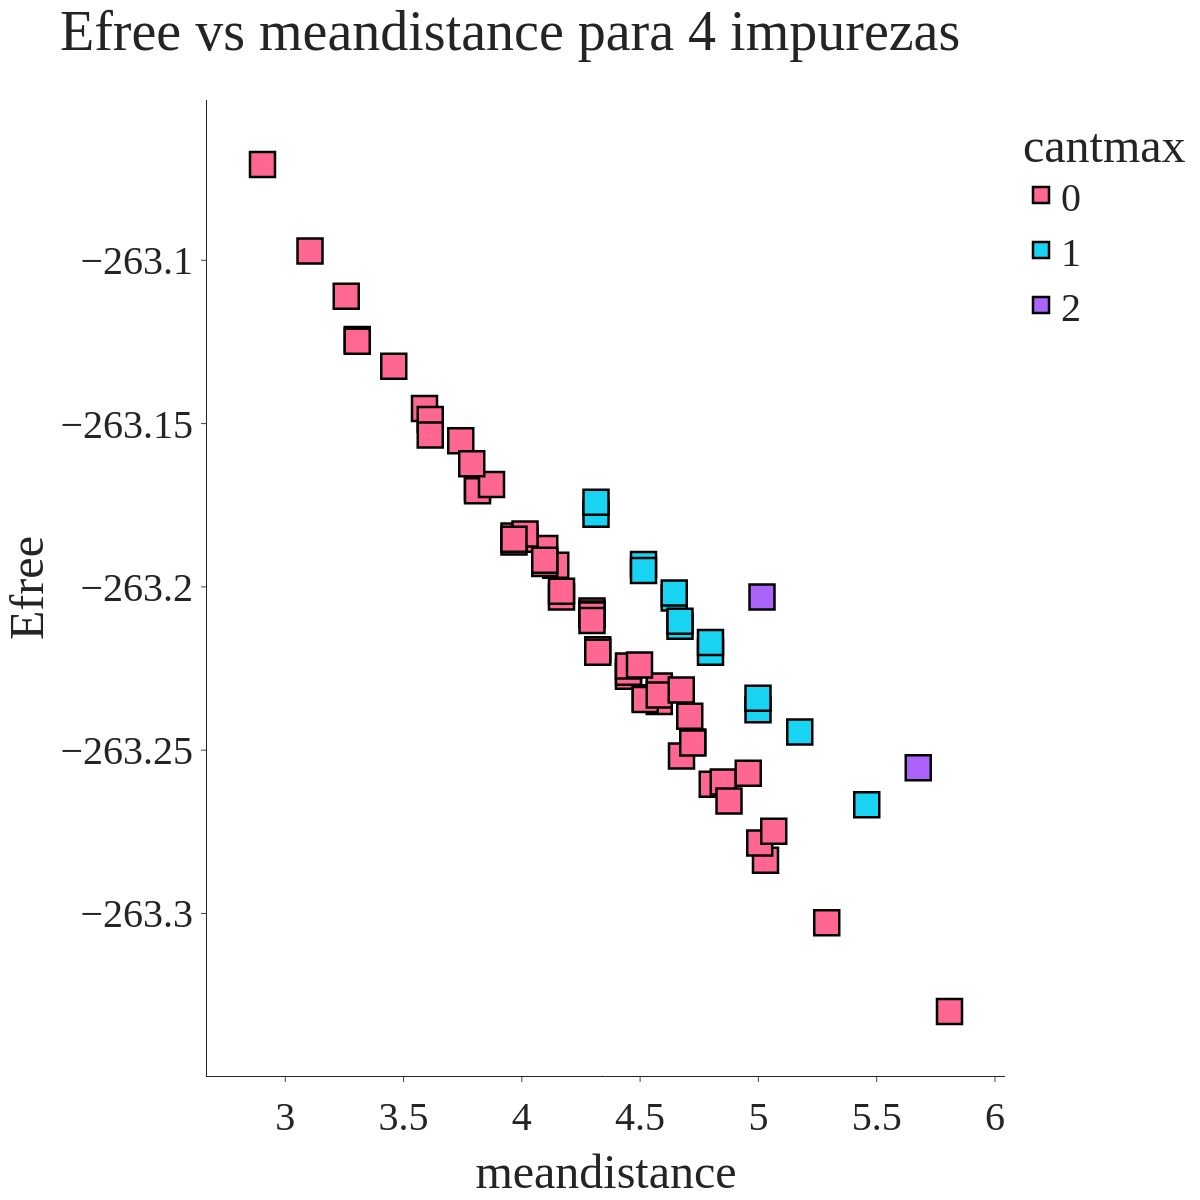
\includegraphics[width=\textwidth]{images/4_impurezas_cantmax_size10.png}
    \end{minipage}%
    \begin{minipage}[t]{0.5\textwidth}
        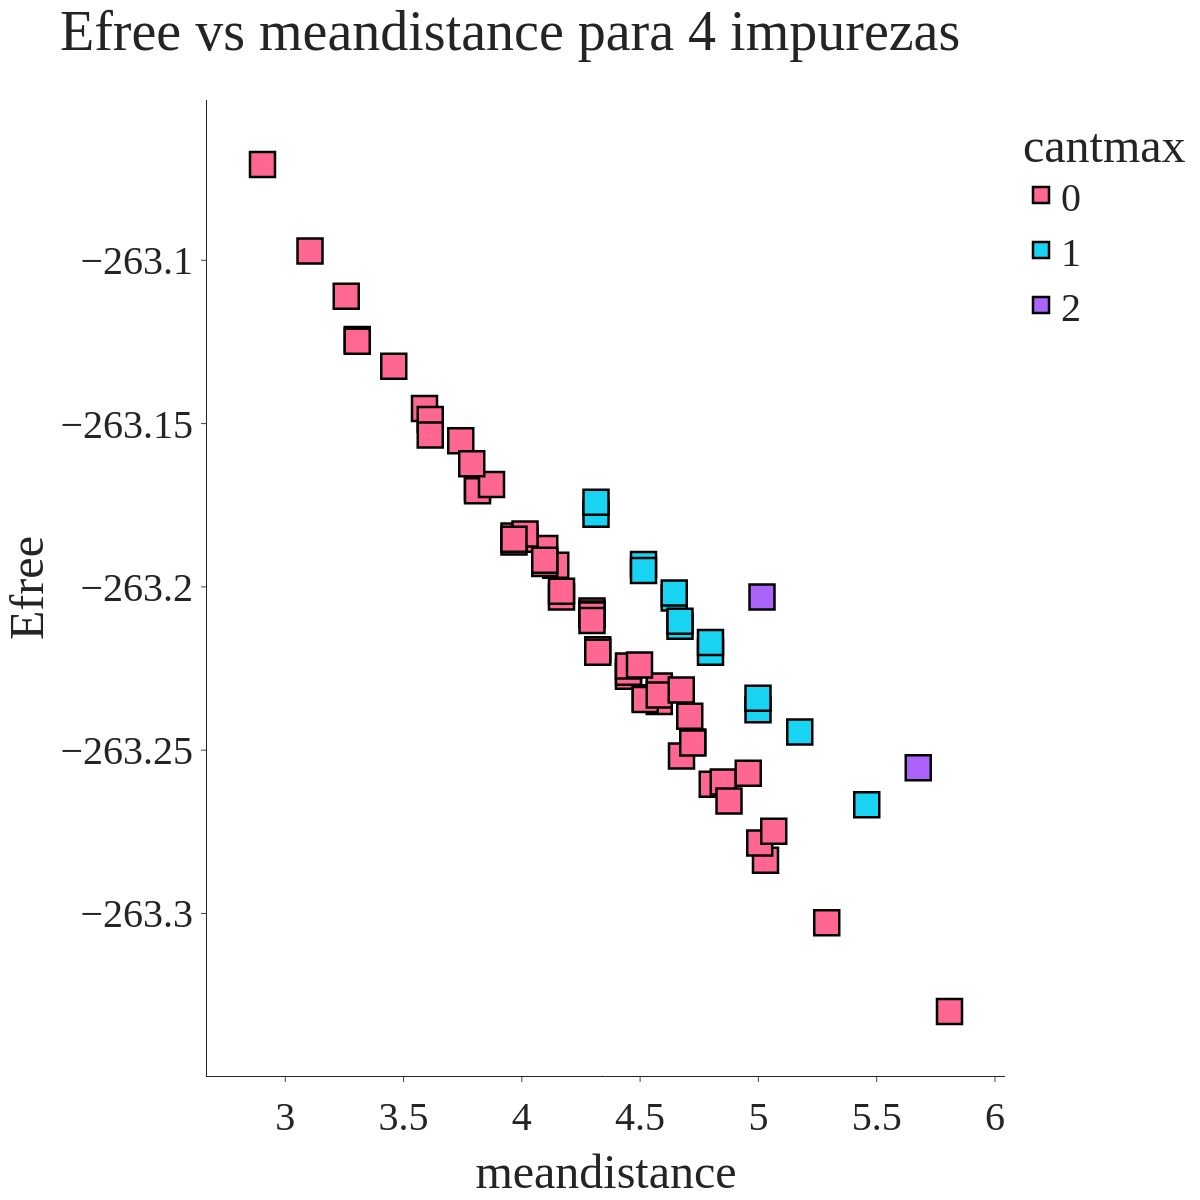
\includegraphics[width=\textwidth]{images/4_impurezas_cantmax_size10.png}    \end{minipage}%
    \caption{Ejemplo de scatterplot hecho con matplotlib.}
    \label{fig:scatterplot_3}
\end{figure}





\begin{mdframed}
    Recuerde que es imprescindible que se pueda replicar la generación de las gráficas, por lo que usted debe incluir cómo generó esos datos y  cómo podría generarlos la persona que revisa su entrega y ejecuta sus programas. Por ejemplo, si genera un scatterpolot con Tikz, usted debe explicar cómo obtener la tupla de valores que se usaron para generar la gráfica.
\end{mdframed}


\newpage
\section{Conclusiones}



\newpage

\section{Condiciones de entrega}
% Condiciones generales de tareas de Algoritmos y Complejidad, 20242
  \begin{itemize}
  \item
    La tarea se realizará \tca{individualmente}
    (esto es grupos de una persona),
    sin excepciones.
  \item
    La entrega debe realizarse vía \url{http://aula.usm.cl}
    en un \tca{tarball} en el área designada al efecto,
    en el formato \tca{\texttt{tarea-\tnum-{rol}.tar.gz}}
    (\texttt{rol} con dígito verificador y sin guión).

    Dicho \tca{tarball} debe contener las fuentes en \LaTeXe{}
    (al menos \tca{\texttt{tarea-\tnum.tex}})
    de la parte escrita de su entrega,
    además de un archivo \tca{\texttt{tarea-\tnum.pdf}},
    correspondiente a la compilación de esas fuentes.
  \item Si se utiliza algún código, idea, o contenido extraído de otra fuente, este \textbf{debe} ser citado en el lugar exacto donde se utilice, en lugar de mencionarlo al final del informe. 
  \item
    Asegúrese que todas sus entregas tengan sus datos completos:
    número de la tarea, ramo, semestre, nombre y rol.
    Puede incluirlas como comentarios en sus fuentes \LaTeX{}
    (en \TeX{} comentarios son desde \% hasta el final de la línea)
    o en posibles programas.
    Anótese como autor de los textos.
 
  \item
    Si usa material adicional al discutido en clases,
    detállelo.
    Agregue información suficiente para ubicar ese material
    (en caso de no tratarse de discusiones con compañeros de curso
     u otras personas).
  \item No modifique \texttt{preamble.tex}, \texttt{tarea\_main.tex}, \texttt{condiciones.tex}, estructura de directorios, nombres de archivos, configuración del documento, etc. Sólo agregue texto, imágenes, tablas, código, etc. En el códigos funte de su informe, no agregue paquetes, ni archivos .tex (a excepción de que agregue archivos en \texttt{/tikz}, donde puede agregar archivos .tex con las fuentes de gráficos en \texttt{TikZ}).

\ifprograms
  \item
    Su programa ejecutable debe llamarse \tca{\texttt{tarea\tnum}},
    de haber varias preguntas solicitando programas,
    estos deben llamarse usando el número de la pregunta,
    como \tca{\texttt{tarea\tnum-1}},
    \tca{\texttt{tarea\tnum-2}},
    etc.
    Si hay programas compilados, con en este caso,
    incluya una \tca{\texttt{Makefile}}
    que efectúe las compilaciones correspondientes.

    Los programas se evalúan según que tan claros
    (bien escritos)
    son, si se compilan y ejecutan sin errores o advertencias según corresponda.
    Parte del puntaje es por ejecución correcta con casos de prueba.
    Si el programa no se ciñe a los requerimientos de entrada y salida,
    la nota respectiva es cero.
\fi    
  \item
    %La entrega debe realizarse dentro del plazo indicado en \url{http://aula.usm.cl}:
    La fecha límite de entrega es el día \tca{10 de noviembre de 2024}.

    \begin{center}
        \Large{
          \textbf{NO SE ACEPTARÁN TAREAS FUERA DE PLAZO}.
        }
        \normalsize
    \end{center}
     
    
  \item
    Nos reservamos el derecho de llamar a interrogación
    sobre algunas de las tareas entregadas.
    En tal caso,
    la nota de la tarea será la obtenida en la interrogación.
    \begin{center}
      \Large{
        \textbf{NO PRESENTARSE A UN LLAMADO A INTERROGACIÓN SIN JUSTIFICACIÓN PREVIA SIGNIFICA AUTOMÁTICAMENTE NOTA 0.}
      }
    \end{center}
    
  \end{itemize}

%%% Local Variables:
%%% mode: latex
%%% ispell-local-dictionary: "spanish"
%%% End:

  
% LocalWords:  tarball tar gz pdf min entregable Makefile puntaje
% LocalWords:  Moodle

\newpage
\appendix





 
\printbibliography

\end{document}


